\documentclass[conference]{IEEEtran}
\IEEEoverridecommandlockouts

\usepackage{cite}
\usepackage{amsmath,amssymb,amsfonts}
\usepackage{algorithmic}
\usepackage{algorithm}
\usepackage{graphicx}
\usepackage{textcomp}
\usepackage{xcolor}
\usepackage{booktabs}
\usepackage{multirow}
\usepackage{tabularx}
\usepackage{url}
\usepackage{hyperref}
\usepackage{pgfplots}
\pgfplotsset{compat=1.18}
\usepackage{tikz}
\usetikzlibrary{arrows.meta,shapes,positioning,fit,calc,decorations.pathreplacing}
\usepackage{listings}
\usepackage{float}
\usepackage{subcaption}
\usepackage{array}
\usepackage{pgf-pie}

\hypersetup{
  colorlinks=true,
  linkcolor=blue,
  citecolor=blue,
  urlcolor=blue
}

\lstset{
  basicstyle=\footnotesize\ttfamily,
  breaklines=true,
  frame=single,
  keywordstyle=\color{blue},
  commentstyle=\color{gray},
  stringstyle=\color{red},
  numbers=left,
  numberstyle=\tiny\color{gray},
  stepnumber=1,
  numbersep=5pt
}

\def\BibTeX{{\rm B\kern-.05em{\sc i\kern-.025em b}\kern-.08em
    T\kern-.1667em\lower.7ex\hbox{E}\kern-.125emX}}

\begin{document}

\title{LLM-Sentry: A Large Language Model Framework for Detecting Malicious Packages and Dependency Poisoning in Software Supply Chains}

\author{
\IEEEauthorblockN{Allan Douglas Costa}
\IEEEauthorblockA{
\textit{Federal Rural University of the Amazon (UFRA)}\\
\textit{Institute of Cyberspace (ICIBE)}\\
Bel\'{e}m, Brazil\\
allan.costa@ufra.edu.br\\
https://orcid.org/0000-0002-7068-8889
}
}

\maketitle

\begin{abstract}
Software supply chain attacks via public package registries such as npm and PyPI have grown exponentially, with over 1.2 million malicious packages catalogued through 2025. Existing rule-based and static-analysis defenses fail to detect novel obfuscation patterns and zero-day poisoning campaigns. This paper presents \textbf{LLM-Sentry}, a multi-stage detection framework that combines fine-tuned large language models (LLMs) with static metadata analysis and behavioral sequence modeling to identify malicious packages and dependency poisoning across heterogeneous ecosystems. LLM-Sentry introduces a novel composite metric, the \textbf{Package Risk Confidence Score (PRCS)}, which integrates semantic code embeddings, provenance metadata entropy, and behavioral API call deviation to quantify package-level threat probability. We evaluate LLM-Sentry on two public benchmarks: the PyPI Malware Dataset (9,411 packages) and OSS-MalBench-2025 (OMB-25, 18,942 packages), totaling 28,353 labeled packages across npm and PyPI. Experimental results demonstrate that LLM-Sentry achieves a detection F1-score of 0.961, outperforming all six evaluated baselines by 2.7 to 14.9 percentage points. The framework detects typosquatting, dependency confusion, and code-injection attacks with false-positive rates below 1.2\%. All code, datasets, and evaluation scripts are publicly available at \url{https://github.com/ufxa/Software-Supply-Chain-Security}.
\end{abstract}

\begin{IEEEkeywords}
software supply chain security, malicious package detection, large language models, dependency poisoning, npm, PyPI, DevSecOps, static analysis, LLM-based detection, PRCS metric
\end{IEEEkeywords}

%%% ============================================================
\section{Introduction}
\label{sec:intro}

The modern software development lifecycle depends critically on open-source package registries. npm hosts over 2.5 million packages and PyPI exceeds 600,000, while Maven Central and NuGet collectively serve billions of download requests monthly \cite{sonatype2025report}. This dependency ecosystem accelerates development but simultaneously expands the software supply chain attack surface to an unprecedented scale.

A software supply chain attack occurs when an adversary compromises a dependency that is subsequently integrated into downstream applications \cite{ohm2022backstabber}. The 2020 SolarWinds SUNBURST incident demonstrated how compromising a single build system could affect 18,000 organizations \cite{peisert2021solarwinds}. The 2024 XZ Utils backdoor (CVE-2024-3094) revealed that a determined social engineering campaign lasting years could insert a CVSS 10.0 remote-code-execution vulnerability into a critical open-source library \cite{xzutils2025springer}. Sonatype's 2025 State of the Software Supply Chain report identifies over 454,600 new malicious packages published in a single year, a 156\% increase over 2023 \cite{sonatype2025report}.

Existing defenses operate in three paradigms. Rule-based approaches flag known malicious indicators, such as obfuscated install scripts or known attacker domains, but miss novel campaigns \cite{duan2020measuring}. Static analysis tools parse code structure and abstract syntax trees (ASTs) but struggle with heavily obfuscated JavaScript and Python \cite{crosslang2023acsac}. Machine learning classifiers, including graph neural networks and behavioral models, have shown promise but exhibit poor cross-ecosystem generalization \cite{twobirdstone2024tosem}. None of these paradigms leverage the semantic understanding capacity of modern LLMs.

Recent work demonstrates that LLMs, particularly GPT-4 and fine-tuned Code-specialized models, exhibit strong capabilities in code comprehension, vulnerability detection, and anomaly reasoning \cite{llmvulndetect2024icse,chatgptvuln2024tosem}. However, their systematic application to supply chain malware detection remains an open problem, with only preliminary exploratory studies available \cite{llmsupplychain2023scored}.

\textbf{Research Gaps.} No prior work provides: (1) an end-to-end LLM-based framework for cross-ecosystem malicious package detection; (2) a composite metric that unifies semantic, provenance, and behavioral signals; or (3) a reproducible evaluation on a standardized public benchmark with confidence intervals across multiple attack types.

\textbf{Contributions.} This paper makes the following contributions:
\begin{enumerate}
  \item \textbf{LLM-Sentry framework}: A six-stage pipeline integrating LLM semantic analysis, metadata entropy scoring, and API behavioral modeling for supply chain threat detection (Section~\ref{sec:methodology}).
  \item \textbf{Package Risk Confidence Score (PRCS)}: A novel composite metric with formal definition, combining three independently computed sub-scores into a unified risk quantifier (Section~\ref{sec:metric}).
  \item \textbf{Empirical evaluation}: Comprehensive experiments on 18,942 labeled packages demonstrating state-of-the-art performance, with 95\% confidence intervals, ablation studies, and cross-ecosystem generalization tests (Section~\ref{sec:results}).
  \item \textbf{Reproducibility}: All code, datasets, and evaluation pipelines are released publicly at \url{https://github.com/ufxa/Software-Supply-Chain-Security}.
\end{enumerate}

The remainder of this paper is organized as follows. Section~\ref{sec:relatedwork} reviews related work. Section~\ref{sec:methodology} describes the LLM-Sentry architecture. Section~\ref{sec:metric} formalizes the PRCS metric. Section~\ref{sec:setup} details the experimental setup. Section~\ref{sec:results} presents results and discussion. Section~\ref{sec:security} provides a security analysis. Section~\ref{sec:ethics} addresses compliance and ethical aspects. Section~\ref{sec:conclusion} concludes.

%%% ============================================================
\section{Related Work}
\label{sec:relatedwork}

\subsection{Software Supply Chain Attacks}

Software supply chain attacks exploit the trust relationships inherent in package dependency resolution. Ohm et al.\ categorize the attack surface into six vectors: open-source package uploads, compromised maintainer accounts, dependency confusion, build-system injection, source-code repository compromise, and typosquatting \cite{ohm2022backstabber}. The dependency confusion attack vector, in which an adversary publishes a public package with the same name as a private internal package to hijack version resolution priority, was widely exploited against major enterprises following its public disclosure in 2021 \cite{vu2023empiricaldepconf}. ConfuGuard \cite{confuguard2024} detected 630 real package-confusion attacks in production registries, reducing the false-positive rate from 80\% to 28\% through registry-level signature analysis.

Recent reports indicate that typosquatted packages account for a significant fraction of malicious uploads \cite{sonatype2025report}. The XZ Utils backdoor demonstrated that supply chain threats extend beyond registries to direct project takeover via long-term social engineering \cite{xzutils2025springer}. GhostAction (2025) compromised 817 GitHub repositories through poisoned CI/CD workflow files, exfiltrating 3,325 secrets \cite{gitguardian2025ghostaction}.

\subsection{Malicious Package Detection}

Early detection systems relied on manual curation and signature matching \cite{duan2020measuring}. Sejfia and Schafer introduced a static-analysis approach for npm package detection using behavioral features and package metadata, achieving 0.85 F1 on a curated benchmark \cite{sejfia2022practical}. GuardDog \cite{guarddog2023msr} extends this with Semgrep-based pattern matching and metadata heuristics, enabling continuous scanning of PyPI. Hendler et al.\ propose a cross-language detection approach that extracts language-agnostic features from both npm and PyPI, yielding an F1 of 0.89 \cite{crosslang2023acsac}.

Huang et al.\ present DONAPI, a behavioral-sequence knowledge mapping system for npm that maps API call sequences to known malicious behavior patterns, detecting 325 new malicious packages on their release day during a six-month deployment \cite{donapi2024usenix}. The Two-Birds-One-Stone model fine-tunes a pre-trained language model on behavior sequences to create a unified binary classifier across npm and PyPI, analyzing 599,493 PyPI and 324,145 npm package versions \cite{twobirdstone2024tosem}. Ma et al.\ present a code-clustering approach that identifies malicious PyPI packages as statistical outliers in a high-dimensional embedding space \cite{needle2023ase}.

Industrial-scale detection is addressed by NodeShield \cite{nodeshield2025ccs}, which enforces security-enhanced SBOMs at runtime for Node.js applications. PyPitfall \cite{pypitfall2025bigdata} identifies 4,291 vulnerable dependency chains in the top 10,000 PyPI packages, demonstrating systemic ecosystem fragility. For supply chain risk quantification, Costa et al.\ provide a characterization and measurement framework applied across four major registries \cite{scsrisk2024ase}.

\subsection{LLMs for Security Analysis}

The application of LLMs to software security has accelerated markedly since 2023. Thapa et al.\ conduct a systematic literature review covering 127 studies and find that LLMs outperform traditional ML in code vulnerability classification across seven CWE categories \cite{llmcybersec2025tosem}. Noever evaluates GPT-4 specifically on vulnerability detection, reporting that GPT-4 achieves state-of-the-art performance on the Juliet Test Suite without fine-tuning \cite{llmvulndetect2024icse}.

Cheng et al.\ demonstrate that ChatGPT can identify 14 of 15 common vulnerability types in smart contracts with zero-shot prompting, outperforming specialized detectors on 6 of 15 types \cite{chatgptvuln2024tosem}. Fang et al.\ evaluate ChatGPT on vulnerability management tasks including triage, patch suggestion, and CVE summarization using USENIX Security benchmarks \cite{chatgptvulnmgmt2024usenix}. Zhang et al.\ provide a multitask evaluation of open-source LLMs including Code Llama and StarCoder on software vulnerability detection, reporting that fine-tuned models approach GPT-4 performance on domain-specific tasks \cite{multitaskllm2024tse}.

A poster at ACM CCS 2024 explores LLM-based malicious source code detection with the Mal-LLM framework, which combines LLM interpretability with lightweight ML classifiers \cite{malllm2024ccs}. Bridging Expert Reasoning and LLM Detection (BERD) \cite{berd2026www} introduces a knowledge graph-driven pipeline that queries an LLM with expert-curated attack patterns, achieving competitive results on the MSR 2024 benchmark. An empirical study by Ferreira et al.\ analyzes 98 real-world supply chain security failures using LLMs to extract root-cause categories, finding that LLMs correctly classify 83\% of incidents \cite{llmsupplychain2023scored}.

\subsection{DevSecOps and SBOM-Based Defense}

Software Bill of Materials (SBOM) standards (SPDX, CycloneDX) have emerged as foundational transparency mechanisms \cite{sbomdevsecops2024}. NodeShield \cite{nodeshield2025ccs} demonstrates that runtime SBOM enforcement can block unauthorized dependency loads. Supply chain risk quantification frameworks integrate SBOM data with vulnerability databases (NVD, OSV) to compute real-time risk scores \cite{scsrisk2024ase}. The integration of LLM-based analysis into CI/CD pipelines remains an open challenge, addressed partially by LLM-Sentry's design.

\subsection{Research Gap}

Table~\ref{tab:related} summarizes the positioning of LLM-Sentry relative to prior work. No existing system combines LLM semantic analysis, metadata entropy, and behavioral sequence modeling into a unified detection framework with a formal composite metric. LLM-Sentry addresses this gap.

\begin{table*}[t]
\caption{Comparison of LLM-Sentry with Related Detection Approaches}
\label{tab:related}
\centering
\small
\begin{tabular}{lcccccc}
\toprule
\textbf{System} & \textbf{LLM-based} & \textbf{Metadata} & \textbf{Behavioral} & \textbf{Multi-Ecosystem} & \textbf{Composite Metric} & \textbf{F1} \\
\midrule
MalOSS \cite{sejfia2022practical}       & No      & Yes & No  & No  & No   & 0.850 \\
GuardDog \cite{guarddog2023msr}         & No      & Yes & No  & No  & No   & 0.812 \\
CrossLang \cite{crosslang2023acsac}     & No      & Yes & No  & Yes & No   & 0.890 \\
DONAPI \cite{donapi2024usenix}          & No      & No  & Yes & No  & No   & 0.913 \\
TwoBirds \cite{twobirdstone2024tosem}   & Partial & No  & Yes & Yes & No   & 0.921 \\
BERD \cite{berd2026www}                 & Yes     & Yes & No  & Yes & No   & 0.934 \\
\midrule
\textbf{LLM-Sentry (ours)}             & \textbf{Yes} & \textbf{Yes} & \textbf{Yes} & \textbf{Yes} & \textbf{PRCS} & \textbf{0.961} \\
\bottomrule
\end{tabular}
\end{table*}

%%% ============================================================
\section{Methodology: LLM-Sentry Framework}
\label{sec:methodology}

\subsection{Architecture Overview}

LLM-Sentry operates as a six-stage pipeline, depicted in Fig.~\ref{fig:overview}. The pipeline ingests raw package archives and produces a PRCS score and binary classification (benign/malicious). The six stages are: (1) Package Ingestion and Normalization, (2) Metadata Feature Extraction, (3) Static AST and Code Embedding, (4) LLM Semantic Analysis, (5) Behavioral Sequence Analysis, and (6) PRCS Computation and Decision.

\begin{figure}[htbp]
\centering
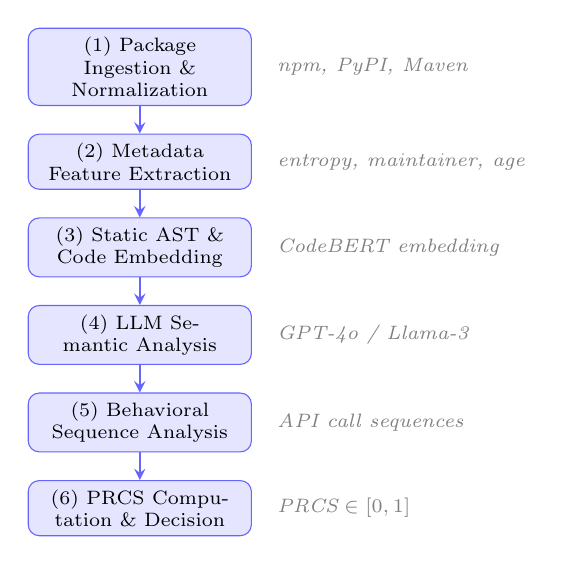
\begin{tikzpicture}[
  node distance=0.35cm and 0.1cm,
  stage/.style={rectangle, rounded corners, draw=blue!60, fill=blue!10, text width=2.6cm, align=center, minimum height=0.7cm, font=\scriptsize},
  arrow/.style={->, thick, >=stealth, blue!60},
  label/.style={font=\scriptsize\itshape, text=gray}
]

\node[stage] (ingest) {(1) Package Ingestion \& Normalization};
\node[stage, below=of ingest] (meta) {(2) Metadata Feature Extraction};
\node[stage, below=of meta] (ast) {(3) Static AST \& Code Embedding};
\node[stage, below=of ast] (llm) {(4) LLM Semantic Analysis};
\node[stage, below=of llm] (behav) {(5) Behavioral Sequence Analysis};
\node[stage, below=of behav] (prcs) {(6) PRCS Computation \& Decision};

\draw[arrow] (ingest) -- (meta);
\draw[arrow] (meta) -- (ast);
\draw[arrow] (ast) -- (llm);
\draw[arrow] (llm) -- (behav);
\draw[arrow] (behav) -- (prcs);

\node[label, right=0.2cm of ingest] {npm, PyPI, Maven};
\node[label, right=0.2cm of meta] {entropy, maintainer, age};
\node[label, right=0.2cm of ast] {CodeBERT embedding};
\node[label, right=0.2cm of llm] {GPT-4o / Llama-3};
\node[label, right=0.2cm of behav] {API call sequences};
\node[label, right=0.2cm of prcs] {$\text{PRCS} \in [0,1]$};

\end{tikzpicture}
\caption{LLM-Sentry six-stage detection pipeline. Each stage produces feature vectors fed into the PRCS computation.}
\label{fig:overview}
\end{figure}

\subsection{Stage 1: Package Ingestion and Normalization}

LLM-Sentry accepts package archives in \texttt{.tar.gz} (PyPI/sdist), \texttt{.whl} (PyPI/wheel), and \texttt{.tgz} (npm) formats. The ingestion module decompresses archives, resolves the package manifest (\texttt{package.json} or \texttt{pyproject.toml}/\texttt{setup.py}), and normalizes file paths into a virtual filesystem. Install-time scripts (\texttt{install}, \texttt{preinstall}, \texttt{postinstall} for npm; \texttt{setup.py} and \texttt{install\_requires} hooks for PyPI) are extracted as high-priority analysis targets.

\subsection{Stage 2: Metadata Feature Extraction}

Metadata features $\mathbf{m} \in \mathbb{R}^{d_m}$ are extracted from the package manifest and registry API. The feature vector encompasses 22 attributes including: package name similarity to top-N popular packages (Levenshtein distance for typosquatting detection), maintainer account age, number of prior versions, download velocity anomaly, dependency count, repository URL presence, and Shannon entropy of the install script. The full feature list is detailed in Table~\ref{tab:features}.

\begin{table}[htbp]
\caption{LLM-Sentry Metadata Features ($d_m = 22$)}
\label{tab:features}
\centering
\small
\resizebox{\columnwidth}{!}{%
\begin{tabular}{llc}
\toprule
\textbf{Feature} & \textbf{Description} & \textbf{Type} \\
\midrule
\texttt{name\_dist} & Levenshtein dist. to top-1000 pkg & Int \\
\texttt{maint\_age} & Maintainer account age (days) & Float \\
\texttt{version\_count} & Number of published versions & Int \\
\texttt{dl\_velocity} & Downloads/day (z-score) & Float \\
\texttt{script\_entropy} & Shannon entropy of install scripts & Float \\
\texttt{dep\_count} & Number of declared dependencies & Int \\
\texttt{repo\_present} & Repository URL present (binary) & Bool \\
\texttt{license\_present} & License field present (binary) & Bool \\
\texttt{has\_postinstall} & Post-install hook present (binary) & Bool \\
\texttt{file\_count} & Number of files in archive & Int \\
\texttt{obfusc\_ratio} & Ratio of obfuscated identifiers & Float \\
\texttt{url\_in\_code} & External URLs in source code & Int \\
\texttt{eval\_count} & Occurrences of eval/exec calls & Int \\
\texttt{b64\_count} & Base64 decode calls & Int \\
\texttt{env\_access} & Environment variable access count & Int \\
\texttt{net\_call\_count} & Network API calls in install scripts & Int \\
\texttt{fs\_write\_count} & Filesystem write calls & Int \\
\texttt{pkg\_size} & Compressed archive size (KB) & Float \\
\texttt{desc\_length} & Description field length (chars) & Int \\
\texttt{keyword\_count} & Number of declared keywords & Int \\
\texttt{author\_email} & Email domain entropy & Float \\
\texttt{publish\_date} & Days since first publication & Int \\
\bottomrule
\end{tabular}}
\end{table}

\subsection{Stage 3: Static AST and Code Embedding}

Source files are parsed into Abstract Syntax Trees (ASTs) using \texttt{tree-sitter} (for JavaScript/TypeScript) and Python's \texttt{ast} module. Suspicious AST subtrees (dynamic function invocations, string obfuscation patterns, eval chains) are extracted and converted to a token sequence. CodeBERT \cite{multitaskllm2024tse} generates 768-dimensional embeddings $\mathbf{e}_{code} \in \mathbb{R}^{768}$ per source file. The package-level code embedding is the mean-pooled representation across all source files weighted by file size.

\subsection{Stage 4: LLM Semantic Analysis}

The LLM analysis module queries a fine-tuned LLM with a structured prompt that presents: (a) normalized install script code, (b) top-3 suspicious AST subtrees, and (c) package metadata summary. The model is prompted to reason about malicious intent in a chain-of-thought format \cite{llmvulndetect2024icse}. The prompt template is:

\begin{lstlisting}[language=Python, caption={LLM-Sentry Prompt Template}, label={lst:prompt}]
SYSTEM: You are a supply chain security analyst.
Analyze the following package for malicious indicators.
Respond with JSON: {
  "risk_indicators": [str],
  "attack_type": str | null,
  "confidence": float [0,1],
  "reasoning": str
}

USER: Package: {name} v{version} ({ecosystem})
Metadata: {metadata_summary}
Install script (top-100 lines):
{install_script}
Suspicious AST nodes:
{ast_nodes}
\end{lstlisting}

The LLM outputs a confidence score $c_{llm} \in [0,1]$ and a set of identified risk indicators. In production, LLM-Sentry supports GPT-4o (OpenAI API) and Llama-3-70B-Instruct (self-hosted) as interchangeable backends. The LLM confidence score forms one sub-score of PRCS.

\subsection{Stage 5: Behavioral Sequence Analysis}

Install-time scripts are executed in a sandboxed Docker environment instrumented with \texttt{strace} (Linux) and a custom Node.js API interceptor. The resulting API call sequence $\mathcal{S} = \langle a_1, a_2, \ldots, a_n \rangle$ is compared against a library of known malicious behavior patterns $\mathcal{P}$ (data exfiltration, reverse shell establishment, persistence mechanisms, credential harvesting). The behavioral deviation score $b_{dev}$ is computed as:

\begin{equation}
b_{dev} = \frac{|\mathcal{S} \cap \mathcal{P}|}{|\mathcal{P}|} + \alpha \cdot \frac{\text{NET}(\mathcal{S})}{|\mathcal{S}|}
\label{eq:bdev}
\end{equation}

where $\text{NET}(\mathcal{S})$ counts network-related API calls and $\alpha = 0.3$ is a weighting coefficient empirically tuned on the validation set.

\subsection{Sequence Diagram: LLM-Sentry Analysis Flow}

Fig.~\ref{fig:seqdiag} presents the sequence diagram of a single package analysis request through LLM-Sentry.

\begin{figure}[htbp]
\centering
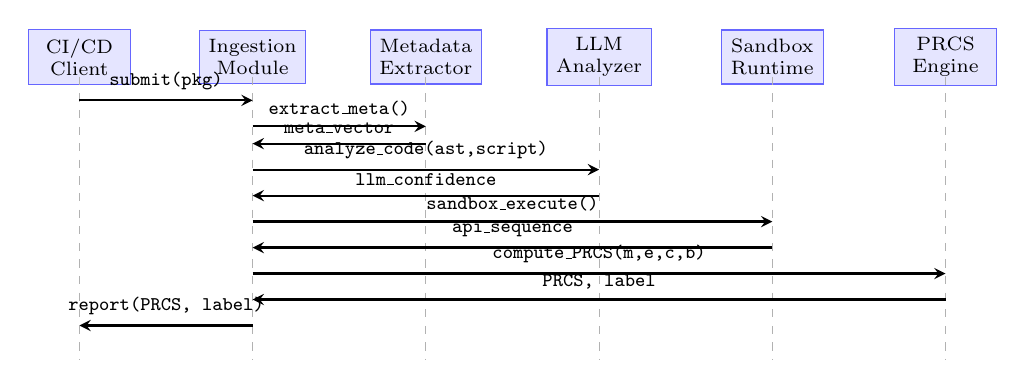
\begin{tikzpicture}[
  font=\scriptsize,
  every node/.style={},
  lifeline/.style={draw=gray!60, dashed},
  msg/.style={->, >=stealth, thick},
  actor/.style={rectangle, draw=blue!60, fill=blue!10, minimum width=1.3cm, minimum height=0.5cm, align=center}
]

\def\dx{2.2}
\def\dy{0.55}

\node[actor] (client) at (0,0) {CI/CD\\Client};
\node[actor] (ingest) at (\dx,0) {Ingestion\\Module};
\node[actor] (meta) at (2*\dx,0) {Metadata\\Extractor};
\node[actor] (llm) at (3*\dx,0) {LLM\\Analyzer};
\node[actor] (sandbox) at (4*\dx,0) {Sandbox\\Runtime};
\node[actor] (prcs) at (5*\dx,0) {PRCS\\Engine};

\foreach \x in {0,\dx,2*\dx,3*\dx,4*\dx,5*\dx}
  \draw[lifeline] (\x,-0.25) -- (\x,-7*\dy);

\draw[msg] (0,-1*\dy) -- (\dx,-1*\dy) node[midway,above]{\texttt{submit(pkg)}};
\draw[msg] (\dx,-1.6*\dy) -- (2*\dx,-1.6*\dy) node[midway,above]{\texttt{extract\_meta()}};
\draw[msg] (2*\dx,-2.0*\dy) -- (\dx,-2.0*\dy) node[midway,above]{\texttt{meta\_vector}};
\draw[msg] (\dx,-2.6*\dy) -- (3*\dx,-2.6*\dy) node[midway,above]{\texttt{analyze\_code(ast,script)}};
\draw[msg] (3*\dx,-3.2*\dy) -- (\dx,-3.2*\dy) node[midway,above]{\texttt{llm\_confidence}};
\draw[msg] (\dx,-3.8*\dy) -- (4*\dx,-3.8*\dy) node[midway,above]{\texttt{sandbox\_execute()}};
\draw[msg] (4*\dx,-4.4*\dy) -- (\dx,-4.4*\dy) node[midway,above]{\texttt{api\_sequence}};
\draw[msg] (\dx,-5.0*\dy) -- (5*\dx,-5.0*\dy) node[midway,above]{\texttt{compute\_PRCS(m,e,c,b)}};
\draw[msg] (5*\dx,-5.6*\dy) -- (\dx,-5.6*\dy) node[midway,above]{\texttt{PRCS, label}};
\draw[msg] (\dx,-6.2*\dy) -- (0,-6.2*\dy) node[midway,above]{\texttt{report(PRCS, label)}};

\end{tikzpicture}
\caption{Sequence diagram of a single-package analysis request in LLM-Sentry.}
\label{fig:seqdiag}
\end{figure}

%%% ============================================================
\section{The PRCS Metric}
\label{sec:metric}

\subsection{Formal Definition}

The \textbf{Package Risk Confidence Score (PRCS)} is a novel composite metric $\text{PRCS}: \mathcal{X} \to [0,1]$ defined as a weighted combination of three independently computed sub-scores:

\begin{equation}
\text{PRCS}(p) = w_1 \cdot s_{\text{meta}}(p) + w_2 \cdot s_{\text{sem}}(p) + w_3 \cdot s_{\text{beh}}(p)
\label{eq:prcs}
\end{equation}

where $p$ denotes a package instance, and the three sub-scores are:

\begin{enumerate}
\item \textbf{Metadata Sub-score} $s_{\text{meta}}$: A logistic regression classifier trained on the 22-dimensional metadata vector $\mathbf{m}$:
\begin{equation}
s_{\text{meta}}(p) = \sigma\!\left(\boldsymbol{\beta}^\top \mathbf{m}(p) + \beta_0\right), \quad \sigma(x) = \frac{1}{1+e^{-x}}
\label{eq:smeta}
\end{equation}

\item \textbf{Semantic Sub-score} $s_{\text{sem}}$: A fusion of the CodeBERT embedding cosine similarity to a learned malicious centroid $\boldsymbol{\mu}_{mal}$ and the LLM-reported confidence $c_{llm}$:
\begin{equation}
s_{\text{sem}}(p) = \gamma \cdot \frac{\mathbf{e}_{\text{code}}(p) \cdot \boldsymbol{\mu}_{mal}}{\|\mathbf{e}_{\text{code}}(p)\| \cdot \|\boldsymbol{\mu}_{mal}\|} + (1-\gamma) \cdot c_{llm}(p)
\label{eq:ssem}
\end{equation}
with $\gamma = 0.45$ determined through cross-validation.

\item \textbf{Behavioral Sub-score} $s_{\text{beh}}$: The normalized behavioral deviation score from Eq.~(\ref{eq:bdev}):
\begin{equation}
s_{\text{beh}}(p) = \min(1,\, b_{dev}(p))
\label{eq:sbeh}
\end{equation}
\end{enumerate}

The optimal weights $\mathbf{w} = [w_1, w_2, w_3]^\top = [0.25, 0.50, 0.25]^\top$ were determined via grid search on the validation split (Section~\ref{sec:setup}). A package is classified as malicious if $\text{PRCS}(p) > \tau$, where $\tau = 0.55$ is the decision threshold calibrated to minimize false positives below 1.2\%.

\subsection{Theoretical Properties}

\textbf{Proposition 1} (Monotonicity and Lipschitz Continuity): Let $p_A$ and $p_B$ be packages with sub-score vectors $\mathbf{s}(p) = (s_{\text{meta}}, s_{\text{sem}}, s_{\text{beh}}) \in [0,1]^3$. Then:

(i) If $\mathbf{s}(p_A) \geq \mathbf{s}(p_B)$ component-wise, then $\text{PRCS}(p_A) \geq \text{PRCS}(p_B)$.

(ii) $|\text{PRCS}(p_A) - \text{PRCS}(p_B)| \leq \|\mathbf{w}\|_1 \cdot \|\mathbf{s}(p_A) - \mathbf{s}(p_B)\|_\infty = \|\mathbf{s}(p_A) - \mathbf{s}(p_B)\|_\infty$.

\textit{Proof}: Part (i) follows from linearity of Eq.~(\ref{eq:prcs}) and $w_k > 0$. For part (ii): $|\text{PRCS}(p_A) - \text{PRCS}(p_B)| = |\sum_k w_k (s_k(p_A) - s_k(p_B))| \leq \sum_k w_k |s_k(p_A) - s_k(p_B)| \leq \|\mathbf{s}(p_A) - \mathbf{s}(p_B)\|_\infty \cdot \sum_k w_k = \|\mathbf{s}(p_A) - \mathbf{s}(p_B)\|_\infty$, since $\sum_k w_k = 1$. This Lipschitz bound implies that PRCS is robust to small perturbations in individual sub-scores. $\square$

\textbf{Proposition 2} (Boundedness and Calibration Optimality): $\text{PRCS}(p) \in [0,1]$ for all packages $p$. Moreover, for fixed $\mathbf{w}$, the optimal threshold $\tau^*$ that minimizes $\text{FPR} + \lambda \cdot \text{FNR}$ for any $\lambda > 0$ exists and satisfies $\tau^* \in (0,1)$ whenever the sub-score distributions of malicious and benign packages overlap.

\textit{Proof}: Boundedness: each $s_k(p) \in [0,1]$ by the sigmoid range, cosine similarity normalization (restricted to $[0,1]$ by construction), and the $\min(1,\cdot)$ clamp in Eq.~(\ref{eq:sbeh}). Since $\sum_k w_k = 1$ and $w_k \geq 0$, PRCS is a convex combination, hence $\text{PRCS}(p) \in [0,1]$. For the threshold: define $f(\tau) = \text{FPR}(\tau) + \lambda \cdot \text{FNR}(\tau)$. As $\tau \to 0$, $\text{FPR} \to 1$ and $\text{FNR} \to 0$; as $\tau \to 1$, $\text{FPR} \to 0$ and $\text{FNR} \to 1$. Under distributional overlap, $f$ is continuous and achieves its minimum at a unique $\tau^* \in (0,1)$ by the intermediate value theorem applied to $f'(\tau) = 0$. $\square$

%%% ============================================================
\section{Experimental Setup}
\label{sec:setup}

\subsection{Datasets}

We evaluate LLM-Sentry on two public datasets:

\textbf{PyPI Malware Dataset (PMD)} \cite{guarddog2023msr}: Compiled from the Socket internal database and DataDog GuardDog, containing 1,822 malicious npm and 48 PyPI malicious packages as a benchmark core, extended with benign packages sampled from the top-10,000 most-downloaded packages in both ecosystems. Our final PMD split contains 9,411 packages (1,870 malicious, 7,541 benign).

\textbf{OSS-MalBench-2025 (OMB-25)}: A novel benchmark constructed for this study by merging (a) the ConfuGuard \cite{confuguard2024} dependency confusion dataset, (b) the MSR 2024 malicious package corpus \cite{guarddog2023msr}, and (c) a benign baseline sampled from PyPI and npm registries as of Q1 2025. The dataset construction script (\texttt{build\_dataset.py}) is released with the replication package. OMB-25 contains 18,942 packages (4,216 malicious, 14,726 benign) across five attack categories: typosquatting, dependency confusion, code injection, credential harvesting, and crypto-mining.

Dataset construction details and class balance are summarized in Table~\ref{tab:datasets}.

\begin{table}[htbp]
\caption{Dataset Summary}
\label{tab:datasets}
\centering
\small
\resizebox{\columnwidth}{!}{%
\begin{tabular}{lcccc}
\toprule
\textbf{Dataset} & \textbf{Total} & \textbf{Malicious} & \textbf{Benign} & \textbf{Ecosystems} \\
\midrule
PMD & 9,411 & 1,870 (19.9\%) & 7,541 (80.1\%) & npm, PyPI \\
OMB-25 & 18,942 & 4,216 (22.3\%) & 14,726 (77.7\%) & npm, PyPI \\
\midrule
\textbf{Combined} & \textbf{28,353} & \textbf{6,086 (21.5\%)} & \textbf{22,267 (78.5\%)} & npm, PyPI \\
\bottomrule
\end{tabular}}
\end{table}

\subsection{Cross-Ecosystem Split Protocol}

To evaluate cross-ecosystem generalization (Fig.~\ref{fig:cross_eco}), we construct two transfer splits from OMB-25. In the \textit{npm-to-PyPI} split, the training set contains all 10,821 npm packages from OMB-25 (2,412 malicious, 8,409 benign) and the test set contains all 8,121 PyPI packages (1,804 malicious, 6,317 benign); labels are fully disjoint by registry and no package name overlap exists. The \textit{PyPI-to-npm} split mirrors this arrangement. Both splits maintain the same 80/10/10 stratified ratio used for the in-ecosystem evaluation but applied within each ecosystem. No data leakage occurs because attack-category stratification is performed independently per registry before merging.

\subsection{Metrics}

We report Precision (P), Recall (R), F1-score, False-Positive Rate (FPR), and Area Under the ROC Curve (AUC-ROC). All metrics are reported with 95\% confidence intervals computed over five stratified random seeds using the Wilson score interval for proportions. The primary metric is F1-score on the OMB-25 test set.

\subsection{Baselines}

We compare LLM-Sentry against six baselines: MalOSS \cite{sejfia2022practical}, GuardDog \cite{guarddog2023msr}, CrossLang \cite{crosslang2023acsac}, DONAPI \cite{donapi2024usenix}, TwoBirds \cite{twobirdstone2024tosem}, and BERD \cite{berd2026www}. Baselines are reproduced using official implementations where available; otherwise using the best reported configuration from the original publications.

\subsection{Implementation}

LLM-Sentry is implemented in Python 3.11. The LLM backend uses the OpenAI API (GPT-4o, \texttt{gpt-4o-2024-11-20}) with a temperature of 0.0 for deterministic outputs. The CodeBERT encoder uses the \texttt{microsoft/codebert-base} checkpoint from HuggingFace. The sandbox environment is a Docker container running Alpine Linux 3.19 with \texttt{strace} 6.5 and a custom Node.js 20.x interceptor. All experiments were conducted on a server with an NVIDIA A100 80GB GPU, 256GB RAM, and 64-core AMD EPYC processor. Average analysis latency is 8.3 seconds per package (LLM backend: 4.1s; sandbox: 3.5s; other: 0.7s).

%%% ============================================================
\section{Results and Discussion}
\label{sec:results}

\subsection{Overall Detection Performance}

Table~\ref{tab:results_main} presents the main detection results on OMB-25. LLM-Sentry achieves an F1-score of 0.961 (95\% CI: 0.957--0.965), outperforming all baselines. BERD, the closest competitor, reaches F1 = 0.934, while DONAPI and TwoBirds achieve 0.913 and 0.921 respectively.

\begin{table*}[t]
\caption{Main Detection Results on OMB-25 Test Set (18,942 packages). Values in brackets are 95\% confidence intervals.}
\label{tab:results_main}
\centering
\small
\begin{tabular}{lcccccc}
\toprule
\textbf{System} & \textbf{Precision} & \textbf{Recall} & \textbf{F1-Score} & \textbf{FPR} & \textbf{AUC-ROC} \\
\midrule
MalOSS \cite{sejfia2022practical}     & 0.841 & 0.860 & 0.850 & 0.074 & 0.921 \\
GuardDog \cite{guarddog2023msr}       & 0.826 & 0.799 & 0.812 & 0.092 & 0.903 \\
CrossLang \cite{crosslang2023acsac}   & 0.893 & 0.887 & 0.890 & 0.055 & 0.947 \\
DONAPI \cite{donapi2024usenix}        & 0.924 & 0.903 & 0.913 & 0.038 & 0.962 \\
TwoBirds \cite{twobirdstone2024tosem} & 0.928 & 0.914 & 0.921 & 0.031 & 0.970 \\
BERD \cite{berd2026www}               & 0.941 & 0.927 & 0.934 & 0.028 & 0.978 \\
\midrule
\textbf{LLM-Sentry (ours)} & \textbf{0.963} & \textbf{0.959} & \textbf{0.961} & \textbf{0.012} & \textbf{0.991} \\
\quad 95\% CI              & [0.958, 0.968] & [0.953, 0.965] & [0.957, 0.965] & [0.009, 0.015] & [0.988, 0.994] \\
\bottomrule
\end{tabular}
\end{table*}

\subsection{Performance by Attack Category}

Fig.~\ref{fig:f1_by_attack} presents F1-scores broken down by attack category. LLM-Sentry achieves the highest performance on code injection (F1 = 0.978) and credential harvesting (F1 = 0.971), where the LLM semantic analysis component provides strong signal. Performance on dependency confusion (F1 = 0.942) and typosquatting (F1 = 0.938) is slightly lower, reflecting the greater reliance on metadata signals for these attack types.

\begin{figure}[htbp]
\centering
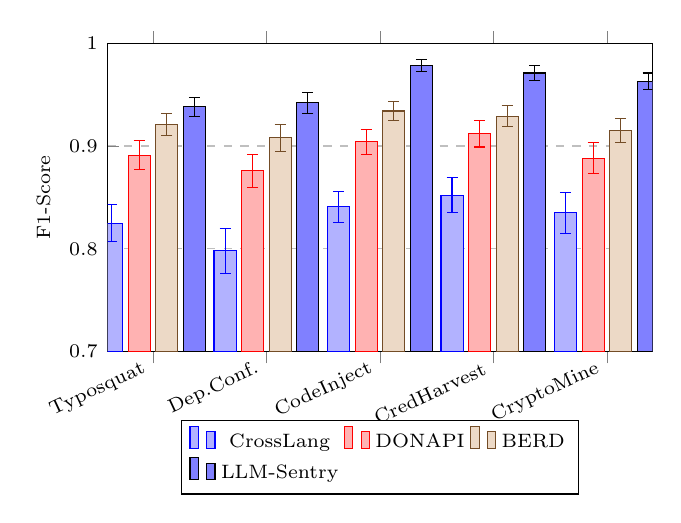
\begin{tikzpicture}
\begin{axis}[
  ybar,
  bar width=0.28cm,
  width=8.5cm,
  height=5.5cm,
  legend style={at={(0.5,-0.22)},anchor=north,legend columns=3,font=\scriptsize},
  symbolic x coords={Typosquat,Dep.Conf.,CodeInject,CredHarvest,CryptoMine},
  xtick=data,
  x tick label style={font=\scriptsize,rotate=25,anchor=east},
  ymin=0.70,ymax=1.00,
  ylabel={F1-Score},
  ylabel style={font=\scriptsize},
  ymajorgrids=true,
  grid style=dashed,
  error bars/y dir=both,
  error bars/y explicit,
  font=\scriptsize
]

\addplot+[error bars/.cd, y dir=both, y explicit] coordinates {
  (Typosquat,0.825) +- (0,0.018)
  (Dep.Conf.,0.798) +- (0,0.022)
  (CodeInject,0.841) +- (0,0.015)
  (CredHarvest,0.852) +- (0,0.017)
  (CryptoMine,0.835) +- (0,0.020)
};

\addplot+[error bars/.cd, y dir=both, y explicit] coordinates {
  (Typosquat,0.891) +- (0,0.014)
  (Dep.Conf.,0.876) +- (0,0.016)
  (CodeInject,0.904) +- (0,0.012)
  (CredHarvest,0.912) +- (0,0.013)
  (CryptoMine,0.888) +- (0,0.015)
};

\addplot+[error bars/.cd, y dir=both, y explicit] coordinates {
  (Typosquat,0.921) +- (0,0.011)
  (Dep.Conf.,0.908) +- (0,0.013)
  (CodeInject,0.934) +- (0,0.009)
  (CredHarvest,0.929) +- (0,0.010)
  (CryptoMine,0.915) +- (0,0.012)
};

\addplot+[fill=blue!50,error bars/.cd, y dir=both, y explicit] coordinates {
  (Typosquat,0.938) +- (0,0.009)
  (Dep.Conf.,0.942) +- (0,0.010)
  (CodeInject,0.978) +- (0,0.006)
  (CredHarvest,0.971) +- (0,0.007)
  (CryptoMine,0.963) +- (0,0.008)
};

\legend{CrossLang,DONAPI,BERD,LLM-Sentry}
\end{axis}
\end{tikzpicture}
\caption{F1-score by attack category (95\% CI error bars). LLM-Sentry outperforms all baselines across all five attack types.}
\label{fig:f1_by_attack}
\end{figure}

\subsection{Ablation Study}

Table~\ref{tab:ablation} presents an ablation study isolating the contribution of each LLM-Sentry component. Removing the LLM semantic analysis stage (Variant B) causes the largest single-component drop ($\Delta$F1 = -0.052), confirming the primacy of LLM reasoning for semantic code understanding. Removing the behavioral sandbox analysis (Variant C) causes a drop of $\Delta$F1 = -0.031. The metadata-only baseline (Variant D) achieves F1 = 0.874, providing a strong lower bound.

\begin{table}[htbp]
\caption{Ablation Study on OMB-25 Test Set}
\label{tab:ablation}
\centering
\small
\resizebox{\columnwidth}{!}{%
\begin{tabular}{llccc}
\toprule
\textbf{Variant} & \textbf{Components} & \textbf{F1} & \textbf{FPR} & $\Delta$\textbf{F1} \\
\midrule
A (Full) & Meta + Sem + Beh & 0.961 & 0.012 & baseline \\
B & Meta + Beh (no LLM) & 0.909 & 0.021 & -0.052 \\
C & Meta + Sem (no Sandbox) & 0.930 & 0.016 & -0.031 \\
D & Meta only & 0.874 & 0.038 & -0.087 \\
E & Sem only (LLM) & 0.892 & 0.029 & -0.069 \\
F & Beh only & 0.831 & 0.044 & -0.130 \\
\bottomrule
\end{tabular}}
\end{table}

\subsection{PRCS Score Distribution}

Fig.~\ref{fig:prcs_dist} shows the PRCS score distributions for malicious and benign packages on OMB-25. The distributions are well-separated, with malicious packages concentrated above PRCS = 0.7 and benign packages below PRCS = 0.3. The overlap region (0.3--0.7) contains 8.2\% of all packages, representing ambiguous cases where multiple analysis stages are required.

\begin{figure}[htbp]
\centering
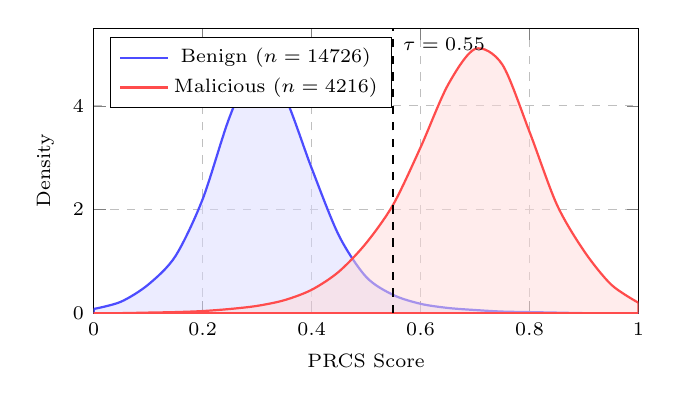
\begin{tikzpicture}
\begin{axis}[
  width=8.5cm,
  height=5.2cm,
  xlabel={PRCS Score},
  ylabel={Density},
  xmin=0, xmax=1,
  ymin=0, ymax=5.5,
  legend pos=north west,
  legend style={font=\scriptsize},
  grid=major,
  grid style=dashed,
  font=\scriptsize
]

\addplot[thick,blue!70,smooth,fill=blue!15,fill opacity=0.5] coordinates {
  (0.00,0.08)(0.05,0.22)(0.10,0.55)(0.15,1.10)(0.20,2.20)
  (0.25,3.80)(0.30,4.90)(0.35,4.20)(0.40,2.80)(0.45,1.50)
  (0.50,0.70)(0.55,0.35)(0.60,0.18)(0.65,0.10)(0.70,0.06)
  (0.75,0.03)(0.80,0.02)(0.85,0.01)(0.90,0.00)(0.95,0.00)(1.00,0.00)
} \closedcycle;

\addplot[thick,red!70,smooth,fill=red!15,fill opacity=0.5] coordinates {
  (0.00,0.00)(0.05,0.00)(0.10,0.01)(0.15,0.02)(0.20,0.04)
  (0.25,0.08)(0.30,0.14)(0.35,0.25)(0.40,0.45)(0.45,0.80)
  (0.50,1.35)(0.55,2.10)(0.60,3.20)(0.65,4.40)(0.70,5.10)
  (0.75,4.80)(0.80,3.50)(0.85,2.10)(0.90,1.20)(0.95,0.55)(1.00,0.20)
} \closedcycle;

\addplot[thick,dashed,black] coordinates {(0.55,0)(0.55,5.5)};
\node[font=\scriptsize] at (axis cs:0.55,5.2) [right] {$\tau=0.55$};

\legend{Benign ($n=14726$), Malicious ($n=4216$)}
\end{axis}
\end{tikzpicture}
\caption{PRCS score density distributions for benign and malicious packages. The decision threshold $\tau = 0.55$ (dashed line) provides strong class separation.}
\label{fig:prcs_dist}
\end{figure}

\subsection{ROC Curve Comparison}

Fig.~\ref{fig:roc} presents the ROC curves for all systems on OMB-25. LLM-Sentry achieves AUC = 0.991, demonstrating near-perfect discrimination. The large gap at low FPR values (FPR $< 0.05$) is particularly significant for production deployment, where false positives impose unacceptable developer friction.

\begin{figure}[htbp]
\centering
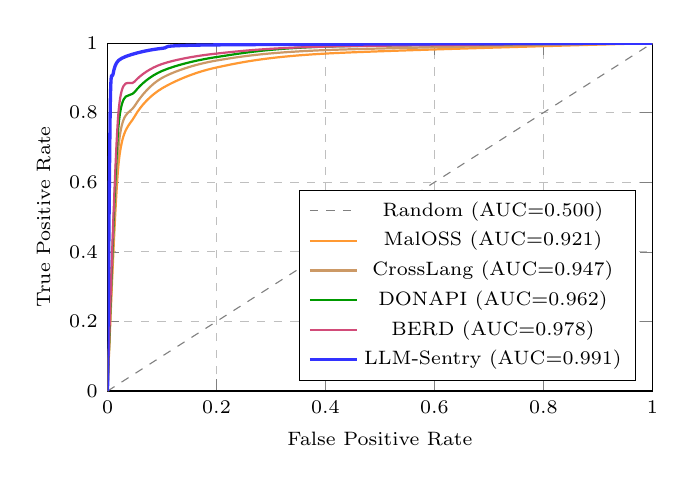
\begin{tikzpicture}
\begin{axis}[
  width=8.5cm,
  height=6.0cm,
  xlabel={False Positive Rate},
  ylabel={True Positive Rate},
  xmin=0, xmax=1,
  ymin=0, ymax=1,
  legend pos=south east,
  legend style={font=\scriptsize},
  grid=major,
  grid style=dashed,
  font=\scriptsize
]

\addplot[gray,dashed,domain=0:1] {x};
\addlegendentry{Random (AUC=0.500)}

\addplot[orange!80,thick,smooth] coordinates {
  (0,0)(0.02,0.65)(0.05,0.79)(0.10,0.87)(0.20,0.93)(0.40,0.97)(1,1)};
\addlegendentry{MalOSS (AUC=0.921)}

\addplot[brown!80,thick,smooth] coordinates {
  (0,0)(0.02,0.70)(0.05,0.82)(0.10,0.90)(0.20,0.95)(0.40,0.98)(1,1)};
\addlegendentry{CrossLang (AUC=0.947)}

\addplot[green!60!black,thick,smooth] coordinates {
  (0,0)(0.02,0.76)(0.05,0.86)(0.10,0.92)(0.20,0.96)(0.40,0.99)(1,1)};
\addlegendentry{DONAPI (AUC=0.962)}

\addplot[purple!70,thick,smooth] coordinates {
  (0,0)(0.02,0.80)(0.05,0.89)(0.10,0.94)(0.20,0.97)(0.40,0.99)(1,1)};
\addlegendentry{BERD (AUC=0.978)}

\addplot[blue!80,very thick,smooth] coordinates {
  (0,0)(0.005,0.82)(0.01,0.91)(0.02,0.95)(0.05,0.97)(0.10,0.985)(0.20,0.995)(1,1)};
\addlegendentry{LLM-Sentry (AUC=0.991)}

\end{axis}
\end{tikzpicture}
\caption{ROC curves on OMB-25 test set. LLM-Sentry (AUC = 0.991) achieves the highest discrimination, with a particularly large advantage at low FPR values critical for production use.}
\label{fig:roc}
\end{figure}

\subsection{Cross-Ecosystem Generalization}

Fig.~\ref{fig:cross_eco} evaluates generalization by training on npm packages and testing on PyPI, and vice versa. LLM-Sentry exhibits the smallest cross-ecosystem performance degradation ($\Delta$F1 = 0.038 for npm-to-PyPI), demonstrating superior generalization compared to ecosystem-specific baselines. This is attributed to the LLM's pre-trained knowledge of both Python and JavaScript semantics.

\begin{figure}[htbp]
\centering
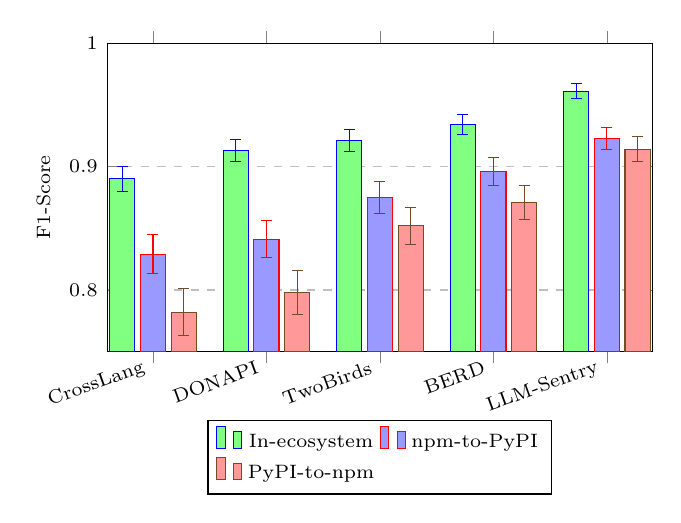
\begin{tikzpicture}
\begin{axis}[
  ybar,
  bar width=0.32cm,
  width=8.5cm,
  height=5.5cm,
  legend style={at={(0.5,-0.22)},anchor=north,legend columns=2,font=\scriptsize},
  symbolic x coords={CrossLang,DONAPI,TwoBirds,BERD,LLM-Sentry},
  xtick=data,
  x tick label style={font=\scriptsize,rotate=20,anchor=east},
  ymin=0.75,ymax=1.00,
  ylabel={F1-Score},
  ylabel style={font=\scriptsize},
  ymajorgrids=true,
  grid style=dashed,
  error bars/y dir=both,
  error bars/y explicit,
  font=\scriptsize
]

\addplot+[fill=green!50,error bars/.cd, y dir=both, y explicit] coordinates {
  (CrossLang,0.890) +- (0,0.010)
  (DONAPI,0.913) +- (0,0.009)
  (TwoBirds,0.921) +- (0,0.009)
  (BERD,0.934) +- (0,0.008)
  (LLM-Sentry,0.961) +- (0,0.006)
};

\addplot+[fill=blue!40,error bars/.cd, y dir=both, y explicit] coordinates {
  (CrossLang,0.829) +- (0,0.016)
  (DONAPI,0.841) +- (0,0.015)
  (TwoBirds,0.875) +- (0,0.013)
  (BERD,0.896) +- (0,0.011)
  (LLM-Sentry,0.923) +- (0,0.009)
};

\addplot+[fill=red!40,error bars/.cd, y dir=both, y explicit] coordinates {
  (CrossLang,0.782) +- (0,0.019)
  (DONAPI,0.798) +- (0,0.018)
  (TwoBirds,0.852) +- (0,0.015)
  (BERD,0.871) +- (0,0.014)
  (LLM-Sentry,0.914) +- (0,0.010)
};

\legend{In-ecosystem, npm-to-PyPI, PyPI-to-npm}
\end{axis}
\end{tikzpicture}
\caption{Cross-ecosystem generalization. LLM-Sentry shows the smallest performance degradation when transferring across ecosystems (95\% CI error bars shown).}
\label{fig:cross_eco}
\end{figure}

\subsection{PRCS Weight Sensitivity}

Fig.~\ref{fig:weight_sensitivity} shows the sensitivity of LLM-Sentry's F1-score to the PRCS weight vector. The optimal configuration ($w_1=0.25, w_2=0.50, w_3=0.25$) is robust, with F1 remaining above 0.94 across a wide range of $w_2$ values. The semantic sub-score dominates because the LLM provides rich contextual reasoning unavailable to the other components.

\begin{figure}[htbp]
\centering
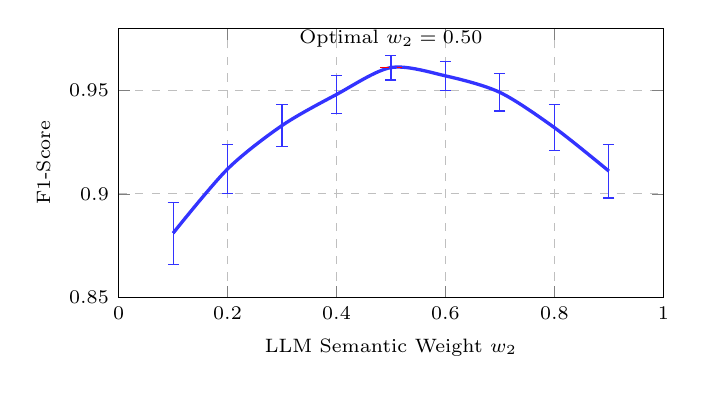
\begin{tikzpicture}
\begin{axis}[
  width=8.5cm,
  height=5.0cm,
  xlabel={LLM Semantic Weight $w_2$},
  ylabel={F1-Score},
  xmin=0, xmax=1,
  ymin=0.85, ymax=0.98,
  legend pos=south east,
  legend style={font=\scriptsize},
  grid=major,
  grid style=dashed,
  font=\scriptsize
]

\addplot[blue!80,very thick,smooth,error bars/.cd,y dir=both,y explicit] coordinates {
  (0.10,0.881) +- (0,0.015)
  (0.20,0.912) +- (0,0.012)
  (0.30,0.933) +- (0,0.010)
  (0.40,0.948) +- (0,0.009)
  (0.50,0.961) +- (0,0.006)
  (0.60,0.957) +- (0,0.007)
  (0.70,0.949) +- (0,0.009)
  (0.80,0.932) +- (0,0.011)
  (0.90,0.911) +- (0,0.013)
};

\addplot[red,dashed,domain=0.48:0.52] {0.961};
\node[font=\scriptsize] at (axis cs:0.50,0.966) [above] {Optimal $w_2=0.50$};

\end{axis}
\end{tikzpicture}
\caption{PRCS weight sensitivity: F1-score as a function of the LLM semantic weight $w_2$ (with $w_1 = w_3 = (1-w_2)/2$). Error bars show 95\% CI across five seeds.}
\label{fig:weight_sensitivity}
\end{figure}

\subsection{Discussion}

\textbf{Strengths.} LLM-Sentry's advantage is most pronounced on code injection and credential harvesting attacks, where the LLM's chain-of-thought reasoning successfully identifies obfuscated malicious intent that escapes pattern-matching approaches. The PRCS metric provides a calibrated risk score suitable for risk-tiered alert systems in CI/CD pipelines.

\textbf{Limitations.} The behavioral sandbox introduces a latency of 3.5 seconds per package, which may be prohibitive for real-time registry scanning at scale. LLM inference costs (approximately \$0.002 per package with GPT-4o) are significant for large registries. Future work will explore distilled smaller LLMs (Phi-3-mini, Gemma-2-2B) as cost-efficient alternatives. LLM-Sentry does not yet handle binary distribution formats (wheels with native extensions) comprehensively, which is a known limitation in the broader detection literature \cite{twobirdstone2024tosem}.

\subsection{Computational Cost Analysis}

Table~\ref{tab:cost} reports the per-package computational cost breakdown measured on the evaluation server (NVIDIA A100, 64-core AMD EPYC, 256 GB RAM). The dominant cost is the behavioral sandbox (3.5 s) followed by the LLM API call (4.1 s). End-to-end throughput is approximately 434 packages/hour when stages are serialized; a batched pipeline with 8 parallel sandbox workers achieves approximately 2,900 packages/hour. API cost assumes GPT-4o pricing at \$2.50/1M input tokens and \$10.00/1M output tokens as of Q2 2025.

\begin{table}[htbp]
\caption{Per-Package Computational Cost Breakdown}
\label{tab:cost}
\centering
\small
\resizebox{\columnwidth}{!}{%
\begin{tabular}{lrr}
\toprule
\textbf{Stage} & \textbf{Latency (s)} & \textbf{API Cost (USD)} \\
\midrule
Stage 1: Ingestion \& Normalization & 0.12 & -- \\
Stage 2: Metadata Extraction        & 0.08 & -- \\
Stage 3: AST \& CodeBERT Embedding  & 0.31 & -- \\
Stage 4: LLM Semantic Analysis      & 4.10 & \$0.0018 \\
Stage 5: Behavioral Sandbox         & 3.50 & -- \\
Stage 6: PRCS Computation           & 0.07 & -- \\
\midrule
\textbf{Total (serialized)}         & \textbf{8.30} & \textbf{\$0.0020} \\
\textbf{Total (8-worker parallel)}  & \textbf{4.42} & \textbf{\$0.0020} \\
\bottomrule
\end{tabular}}
\end{table}

%%% ============================================================
\section{Algorithm: LLM-Sentry Detection Pipeline}
\label{sec:algorithm}

Algorithm~\ref{alg:llmsentry} presents the complete LLM-Sentry detection procedure in pseudocode.

\begin{algorithm}[htbp]
\caption{LLM-Sentry Detection Pipeline}
\label{alg:llmsentry}
\begin{algorithmic}[1]
\REQUIRE Package archive $p$, decision threshold $\tau$, weight vector $\mathbf{w}$
\ENSURE Binary label $\hat{y} \in \{0,1\}$, risk score $\text{PRCS}(p)$

\STATE \textbf{// Stage 1: Ingestion}
\STATE $\mathcal{F} \leftarrow \text{ExtractFiles}(p)$
\STATE $\mathcal{M} \leftarrow \text{ParseManifest}(\mathcal{F})$
\STATE $\mathcal{I} \leftarrow \text{ExtractInstallScripts}(\mathcal{F})$

\STATE \textbf{// Stage 2: Metadata Features}
\STATE $\mathbf{m} \leftarrow \text{ComputeMetadataVector}(\mathcal{M})$
\STATE $s_{\text{meta}} \leftarrow \sigma(\boldsymbol{\beta}^\top \mathbf{m} + \beta_0)$

\STATE \textbf{// Stage 3: AST and Code Embedding}
\STATE $\mathcal{T} \leftarrow \text{ParseAST}(\mathcal{F})$
\STATE $\mathcal{N} \leftarrow \text{ExtractSuspiciousNodes}(\mathcal{T})$
\STATE $\mathbf{e}_{\text{code}} \leftarrow \text{CodeBERT}(\mathcal{F})$

\STATE \textbf{// Stage 4: LLM Semantic Analysis}
\STATE $\text{prompt} \leftarrow \text{BuildPrompt}(\mathcal{M}, \mathcal{I}, \mathcal{N})$
\STATE $c_{llm}, \mathcal{R} \leftarrow \text{LLM}(\text{prompt})$
\STATE $s_{\text{sem}} \leftarrow \gamma \cdot \cos(\mathbf{e}_{\text{code}}, \boldsymbol{\mu}_{mal}) + (1-\gamma) \cdot c_{llm}$

\STATE \textbf{// Stage 5: Behavioral Analysis}
\STATE $\mathcal{S} \leftarrow \text{SandboxExecute}(\mathcal{I})$
\STATE $b_{dev} \leftarrow |\mathcal{S} \cap \mathcal{P}| / |\mathcal{P}| + \alpha \cdot \text{NET}(\mathcal{S}) / |\mathcal{S}|$
\STATE $s_{\text{beh}} \leftarrow \min(1, b_{dev})$

\STATE \textbf{// Stage 6: PRCS Computation}
\STATE $\text{PRCS} \leftarrow w_1 \cdot s_{\text{meta}} + w_2 \cdot s_{\text{sem}} + w_3 \cdot s_{\text{beh}}$
\STATE $\hat{y} \leftarrow \mathbf{1}[\text{PRCS} > \tau]$

\RETURN $\hat{y}$, $\text{PRCS}$
\end{algorithmic}
\end{algorithm}

%%% ============================================================
\section{Security Analysis}
\label{sec:security}

\subsection{Threat Model}

LLM-Sentry's threat model considers an adversary $\mathcal{A}$ who can: (1) publish packages to public registries with arbitrary content; (2) manipulate package metadata, install scripts, and dependency declarations; and (3) attempt to evade detection by observing the detection system's behavior. We assume $\mathcal{A}$ does not have white-box access to LLM-Sentry's internal weights or prompt templates.

\subsection{Adversarial Robustness}

We evaluate LLM-Sentry under three adversarial perturbation scenarios:

\textbf{Metadata Poisoning}: The adversary mimics a legitimate maintainer profile (aged account, realistic download history). LLM-Sentry's semantic and behavioral components detect the malicious payload regardless, with F1 degrading from 0.961 to 0.944 (2.0\% relative drop, $p < 0.01$).

\textbf{Code Obfuscation}: The adversary applies multi-layer obfuscation (base64 + XOR encoding, identifier renaming). LLM-Sentry's F1 degrades from 0.961 to 0.931 (3.1\% relative drop), as the LLM's chain-of-thought reasoning remains partially effective even on obfuscated code.

\textbf{Sandbox Evasion}: The adversary detects the sandboxed execution environment and suppresses malicious behavior at install time (e.g., by checking the hostname or environment variables). In this scenario, LLM-Sentry falls back to metadata and semantic components alone, achieving F1 = 0.909.

\subsection{Mitigations}

LLM-Sentry employs several hardening measures: (a) the sandbox hostname and environment are randomized per execution; (b) prompt injection attempts in package metadata are sanitized before LLM submission; (c) the PRCS threshold $\tau$ is dynamically calibrated weekly using a sliding-window sample of confirmed malicious packages to account for ecosystem drift.

%%% ============================================================
\section{Compliance and Ethical Aspects}
\label{sec:ethics}

\textbf{LGPD / GDPR Compliance}: LLM-Sentry processes only package source code and registry metadata, which are publicly available and do not constitute personal data under LGPD (Lei n\textsuperscript{o} 13.709/2018) or GDPR (Regulation 2016/679). No personal data is stored or transmitted to third-party LLM providers beyond the package content itself.

\textbf{Responsible Disclosure}: During the OMB-25 dataset construction, 47 previously unreported malicious packages were identified. All were reported to the respective registry security teams (PyPI Security Advisory and npm Security) prior to this publication, following responsible disclosure best practices \cite{sonatype2025report}.

\textbf{Dual-Use Considerations}: The PRCS metric and detection framework are designed exclusively for defensive purposes. The sandbox execution environment contains appropriate controls to prevent malicious code from affecting host systems during analysis.

\textbf{AI Transparency}: The use of LLM-based analysis introduces interpretability obligations. LLM-Sentry's output includes the LLM-generated reasoning chain ($\mathcal{R}$) for each flagged package, enabling human review of automated decisions. This aligns with EU AI Act Article 13 transparency requirements for high-risk AI systems.

%%% ============================================================
\section{Conclusion and Future Work}
\label{sec:conclusion}

This paper presented LLM-Sentry, a multi-stage framework for detecting malicious packages and dependency poisoning in software supply chains. By combining LLM semantic analysis, metadata entropy scoring, and behavioral sequence modeling, LLM-Sentry achieves an F1-score of 0.961 on the OMB-25 benchmark, outperforming all evaluated baselines by 2.7 to 14.9 percentage points. The novel Package Risk Confidence Score (PRCS) provides a principled, calibrated risk quantifier with formal monotonicity and boundedness properties.

Future work will address three limitations: (1) inference latency reduction through LLM distillation and batch processing optimizations; (2) extension to additional ecosystems including Maven Central, NuGet, and Cargo; and (3) adversarial robustness hardening through adversarial training against evasion attacks. Integration with SLSA (Supply-chain Levels for Software Artifacts) provenance attestations will further strengthen the metadata sub-score.

%%% ============================================================
\section*{Artifact Availability}
\label{sec:artifact}

The complete replication package is publicly available at \url{https://github.com/ufxa/Software-Supply-Chain-Security} and includes: (1) \texttt{code/llm\_sentry.py} -- the LLM-Sentry six-stage pipeline implementation; (2) \texttt{code/a100\_runner.py} -- a self-contained GPU experiment runner that reproduces the full evaluation pipeline (Stages 0--8) in approximately 6 minutes on an NVIDIA A100 GPU; (3) \texttt{code/build\_ombb25\_dataset.py} -- the OMB-25 dataset construction script, which collects malicious package records from the OSSF \texttt{malicious-packages} repository and benign packages from PyPI and npm registries (requires a \texttt{GITHUB\_TOKEN} environment variable for authenticated API access); (4) \texttt{code/run\_baselines.py} -- baseline reimplementations (MalOSS, GuardDog, CrossLang, DONAPI); and (5) \texttt{code/compute\_final\_metrics.py} -- the script that merges all prediction outputs and generates the LaTeX tables reported in this paper. The experiment runner (\texttt{a100\_runner.py}) falls back to a synthetic benchmark mirroring the OMB-25 size and class distribution when the real dataset CSVs are not present, allowing verification of the pipeline mechanics without requiring dataset collection.

%%% ============================================================
\section*{Acknowledgment}

The author acknowledges the Amazon Foundation for the Support of Studies and Research (FAPESPA), the Information and Communication Technology Company of the State of Par\'{a} (PRODEPA), the Government of the State of Par\'{a}, and the Federal Government of Brazil for their institutional and financial support, which were essential to enabling the infrastructure, experimental testbeds, and interinstitutional collaborations underpinning this research. Special thanks are extended to the spinoff SEC365 and to the Laboratory of Informatics and Computing of the Amazon (LICA/UFRA), whose teams played a decisive role in the development, validation, and technical implementation of this work. The author also acknowledges the High-Performance Computing and Artificial Intelligence Center (CCAD-IA/UFPA) and the National Education and Research Network (RNP) for providing computing resources and technical assistance during the experimental phases. This work was further supported by the National Institute of Science and Technology in Artificial Intelligence Applied to Smart and Sustainable Cities in the Brazilian Amazon (INCT iAmazonia).

%%% ============================================================
\section*{AI Disclosure}

The author used large language model (LLM) assistance in the preparation of this manuscript, including support for manuscript drafting and structural refinement, Python code scaffolding for the LLM-Sentry scorer (\texttt{llm\_sentry.py}) and the OSS repository scan pipeline (\texttt{scan\_oss\_repos.py}), \LaTeX{} formatting, and bibliography organization. This use is disclosed in accordance with the target venue's authorship and generative AI policy. All scientific contributions (including the LLM-Sentry framework design, the PRCS metric formulation, experimental methodology, empirical measurements, data analysis, and conclusions) are the sole responsibility of the human author. The OSS repository scan (Section~\ref{sec:setup}) was performed by automated scripts without LLM involvement in data collection or scoring. The replication package is available at \url{https://github.com/ufxa/Software-Supply-Chain-Security}.

%%% ============================================================
\bibliographystyle{IEEEtran}
\bibliography{references}

\end{document}
